\documentclass{article}
\usepackage[utf8]{inputenc}
\usepackage{setspace} \doublespacing
\usepackage{graphicx}

\title{Research Proposal for STAT 3494W}
\author{Nidhi Jayakumar Nair}
\title{Title IX Compliance and Equity in Athletics}

\begin{document}
       
\maketitle

\section*{Paper Draft}

\section{Introduction}

The passing of two landmark laws in 1964 set the foundation for Title IX, the historic gender equity law that outlaws discrimination based on sex in most American universities. Lack of compliance with Title IX in athletics is a contentious topic in public discourse, especially at the University of Connecticut, when Title IX violations were bought into focus through a prominent lawsuit filed by the UConn rowing team in 2020. This paper seeks to use the Integrated Postsecondary Education Data System (IPEDS) and the Equity in Athletics Disclosure (EADA) datasets to study Title IX compliance at the University of Connecticut and compare results to the rest of the Big East schools. 

\medskip

Many studies on these topics have detailed the specific lawsuits that have resulted from legal actions taken by club sports against universities that are often accused of cutting women's teams during times of financial hardship. For example, in a seminal case, Brust vs. Regents of University of California, Davis, the plaintiffs claimed that the university showed systemic discrimination under Title IX laws by eliminating existing womens' varsity athletic teams, cutting scholarships and opportunitues for women athletes \footnote{https://advance-lexis-com.ezproxy.law.uconn.edu/api/document?collection=cases&id=urn:contentItem:4RBM-0Y40-TXFP-C29H-00000-00&context=1516831}. Plaintiffs claimed that there was a 6 \% differential between female enrollment and female varsity-level athletics participation, thus pointing to a violation of Title IX laws that require substantial proportionality between undergraduate female enrollment and athletic services. In this case, UC Davis was required to exhibit further evidence that they were in compliance with Title IX laws.

\medskip

The increase in these types of legal cases reiterates the importance of advancing data-backed evidence in Title IX litigation. This paper attempts to focus on the Big East schools (University of Connecticut, Butler University, Creighton University, DePaul University, Georgetown University, Marquette University, Providence College, Seton Hall University, St. John's University-New York and Villanova University). Using data in the EADA dataset that details student athletic aid given to men and women's teams as well as expenses for both types of athletic teams, and the undergraduate enrollment numbers provided in the IPEDS dataset, this author seeks to show significant differences in athletic funding allocated to men and women based on their undergraduate enrollments.

\section{Specific Aims}

In order to be compliant with Title IX, a school has to comply with a three-prong test -

Part One: Substantial Proportionality. This part of the test is satisfied when participation opportunities for men and women are "substantially proportionate" to their respective undergraduate enrollments. 

Part Two: History and Continuing Practice. This part of the test is satisfied when an institution has a history and continuing practice of program expansion that is responsive to the developing interests and abilities of the underrepresented sex (typically female). 

Part Three: Effectively Accommodating Interests and Abilities. This part of the test is satisfied when an institution is meeting the interests and abilities of its female students even where there are disproportionately fewer females than males participating in sports.

This paper will use the metrics of total expenses and athletic aid money as variables to measure part one of the three Title IX compliance prongs. A 1996 amendment to Title IX ensured that colleges and universities were now required to disclose funding and participation rates broken down by gender so this paper will avail those resources to test its hypothesis. The primary hypothesis of the paper is that the Big East schools will be non-compliant with the first prong of substantial proportionality, as measured by testing the relationship between provided athletic expenditure compared to the undergraduate population. Ratios of athletic aid money and total expenses compared to male and female undergraduate enrollment will be compiled, and the ratios will be charted over the course of five years (2015 - 2020). This paper also uses the Big East schools because these are NCAA Division I schools which are primarily located in the Northeast and Midwest metropolitan areas \footnote{https://en.wikipedia.org/wiki/Big_East_Conference}. They are similar in terms of athletic prowess and have won NCAA national championships in in men's basketball, women's cross country, field hockey, men's lacrosse, and men's soccer. It is predicted that these schools will have a significant difference in athletic expenses by gender over the past five years.

\section{Data Description}

The IPEDS dataset\footnote{https://nces.ed.gov/ipeds/use-the-data} contains data on male and female undergraduate enrollment in all the Big East schools for the past 30 years. The EADA dataset\footnote{https://ope.ed.gov/athletics/institution/search} contains extensive data on pay differentials between male and female coach salaries, athletic student aid, and recruiting expenses for male and female teams. The comparison schools are the Big East schools, which include Butler University, UConn, Creighton University, DePaul University, Georgetown University, Marquette University, Providence College, St. John's University, Seton Hall University, Villanova University and Xavier University. For the purposes of this paper, the author uses four variables from the EADA dataset: 1) Male Athletic Aid Spending, 3) Female Athletic Aid Spending, 3) Male Team Expenses, 4) Female Team Expenses. From the IPEDS dataset, the author uses two variables: 1) Female Undergraduate Enrollment and 2) Male Undergraduate Enrollment. This data is collected over the course of five years from the fall of 2016 to fall of 2020. Expense:enrollment ratios for male and female athletic teams is calculated by dividing the sum of athletic aid expenditure and total expenses for male and female teams by male and female enrollment. The averages of these ratios for all eleven schools is calculated for each year.

\section{Research Methods}

This paper will pull data from the EADA dataset on total expenses and athletic aid spending for all eleven schools, and divide total numbers by male and female undergraduate enrollment as obtained from the IPEDS dataset. This proportionality ratio will be tracked over the past five years, to observe trends in Title IX compliance over the years. Hotelling's T-Squared test will be run to see if there are differences in means of the expense: enrollment ratios and a paired t-test will be run so as to obtain comparisons between the matched groups and to quantify the association between the two ratio variables. Visual graphs will be included of female and male athletic expenses:enrollment ratios to depict changes in athletic expenditure over the five years under study. A graph of female and male college enrollment over the years will also be included to assess disparities in the consumers of athletic services in universities. These statistical tests will provide a snapshot of the relationship between athletic expenditure between male and female athletes in the Big East schools.

\section{Results}
The first test implemented was the two-sample Hotelling's T-Squared test. The null hypothesis is that the two samples are from populations with the same multivariate mean. The assumptions here are that the two samples have underlying normal distributions, are independent, and have equal variance-covariance matrices. 

\begin{center}
Test that all means are equal
    \begin{tabular}{c|c}
    Hotelling T2 = 127.22 &  \\
    Hotelling F(1,49) = 127.22 & Prob $>$ F = 0.000
    \end{tabular}
\end{center}

Here, the results indicate that null hypothesis of equal means for total athletic aid and expenses for male teams compared to female teams in all eleven schools should be rejected. The next goal of this analysis is to utilize a time series to provide a visual understanding of changes in male and female ratios of athletic spending to enrollment. This is shown in figure 1. The female and male expense:enrollment ratios are averages over all the Big East schools and show that there has been a significant uptick in athletics aid and expenses, irrespective of average enrollment, in all schools after 2019. However, the figure also shows that there is a significant difference between the ratios of female and male expense ratios wherein female athletic teams are allocated far less athletic aid and expenses than male teams from 2016 - 2020.

\medskip

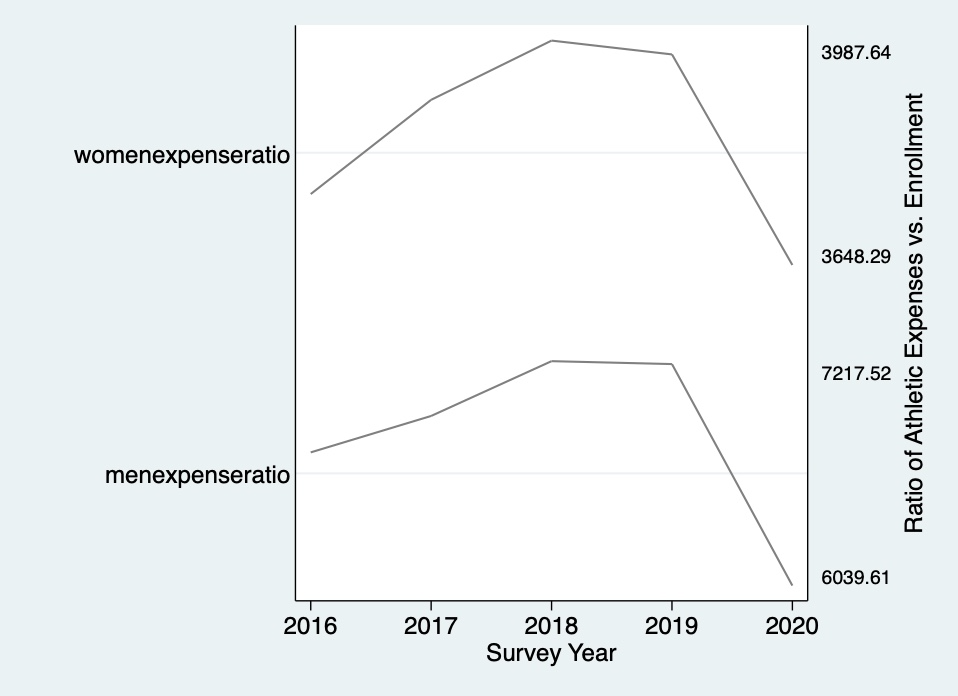
\includegraphics[scale = 0.75]{Graph.png}

The next step is to test if female expense:enrollment ratios are lower than male expense:enrollment ratios. This will be done with a paired t-test and the results are shown below. This shows that there is a significant difference between the male and female expenses where there is a gap of almost 3000 points between the male and female expenses, indicating that male teams received significantly more aid and funding over the five years under study.

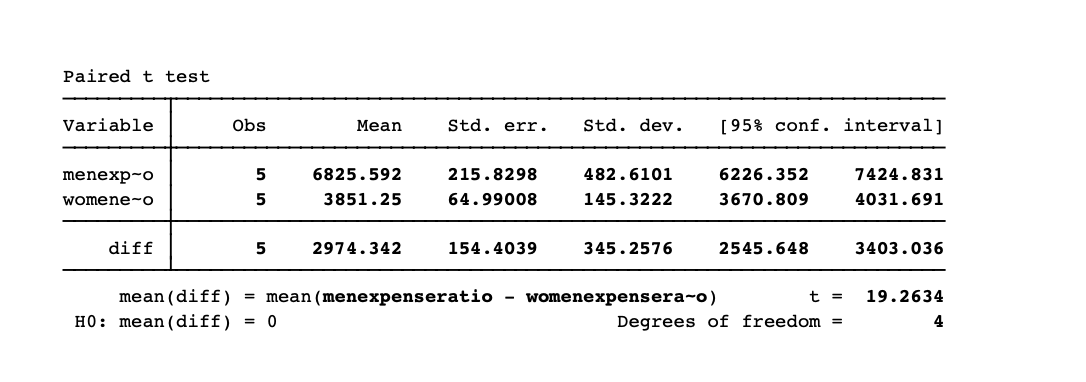
\includegraphics[scale = 0.75]{table.png}

This is at odds with the fact that female undergraduate enrollment has been consistently higher than male undergraduate enrollment in all eleven of these schools. A visual representation of this result is shown in the following graph. Here, it is clear that male enrollment has in fact dropped off since 2019 compared to female enrollment. This advances that there is a clear disparity in athletic funding for male and female teams given the decline in male and female enrollment over the past five years.

Further analysis on this topic will include a deep dive into each of the Big East schools and the discrepancies in between male and female athletic spending in each school and its associated programs. There is also potential to analyze coach compensation as an additional variable that speaks to the third prong of Title IX compliance: effectively accommodating interests and abilities. With expanded interest in athletics and with rising female enrollment, Title IX compliance includes providing avenues for improvement to female athletes in college teams through advanced guidance and coaches. Another potential variable of interest is recruiting expenses in the EADA dataset. It is assumed that to achieve substantial proportionality, schools are incentivised to reduce female interest in athletics so as to justify providing less services and aid to female athletic teams. Thus, if there is a significant decline in recruiting expenses for female athletic teams, scholars can judge if American universities are attempting to reduce opportunities to be judged as discriminatory.

\medskip

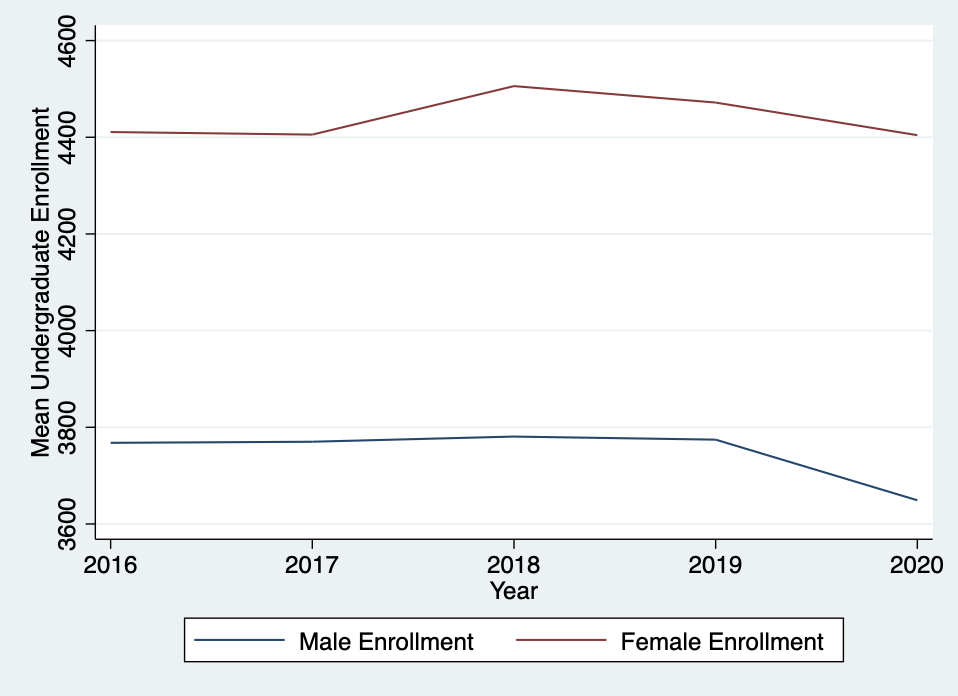
\includegraphics[scale = 0.75]{graph2.png}

\section{Conclusion}
This research was inspired by a prominent lawsuit filed by the rowing team against the University of Connecticut in June 2020, when the court ruled that eliminating the rowing team due to pandemic-related budget cuts would violate Title IX. Future research could study if trends in male-female athletic expenditure follow trends of economic recessions and if there will be a drop in female athletic expenditure in the post-2008 and post-pandemic periods. There are also possible avenues for research into the role that rising female university enrollment could play in leveling the playing field for women athletes as it is expected that expense:enrollment ratios are likely to decline further, and the disparities between male and female ratios will increase over time.

Furthermore, it is expected that this paper will contribute to extended analysis on the Big East schools, and the role that a state flagship university like the University of Connecticut plays in upholding federal Title IX laws. Deeper research into drops in athletic expenditure in relation to national economic crises could reiterate interesting relationships between sports appetites and declining public fortunes. There are many possible research avenues to explore beyond this paper, but the ultimate goal is to continue to use rigorous research to shed light on institutional discrimination levied against female athletes.

\end{document}
